%% The first command in your LaTeX source must be the \documentclass command.
%%
%% Options:
%% twocolumn : Two column layout.
%% hf: enable header and footer.
\documentclass[
twocolumn,
% hf,
]{ceurart}

%%
%% One can fix some overfulls
\sloppy

%%
%% Minted listings support 
%% Need pygment <http://pygments.org/> <http://pypi.python.org/pypi/Pygments>
\usepackage{listings}
%% auto break lines
\lstset{breaklines=true}

\usepackage{blindtext}
\usepackage[linesnumbered,ruled]{algorithm2e}
\usepackage{amsmath}
\usepackage{tikzsymbols}
\usepackage{pifont} % for \ding command
\usepackage{listings}
\usepackage{multirow}
\usepackage{bm}
\usepackage{bbm}
\usepackage{xfrac}
\usepackage{booktabs} % For better horizontal rules
\usepackage{cellspace} % For adjusting vertical spacing
\usepackage{xcolor}
\newcommand\todop[1]{\textcolor{red}{#1}} % todo in the paper
\newcommand\todos[1]{\textcolor{blue}{#1}} % todo in the software
\newcommand{\tik}{\textcolor{green}{\ding{51}}}
\newcommand{\ntik}{\textcolor{red}{\ding{55}}}
\usepackage{lastpage}
\usepackage{caption}
\usepackage{subcaption}

\newcommand{\xcc}{\mathbf{x_{/s}}}
\newcommand{\Xcal}{\mathcal{X}}
\newcommand{\xb}{\mathbf{x}}
\newcommand{\xc}{\mathbf{x_c}}
\newcommand{\Xc}{\mathbf{X_c}}
\newcommand{\xci}{\mathbf{x}^i_c}



%%
%% end of the preamble, start of the body of the document source.
\begin{document}

%%
%% Rights management information.
%% CC-BY is default license.
\copyrightyear{2024}
\copyrightclause{Use permitted under Creative Commons License Attribution 4.0 International (CC BY 4.0).}

%%
%% This command is for the conference information
\conference{2nd International Workshop on Tabular Data Analysis (TaDA) @ VLDB 2024}

%%
%% The "title" command
\title{RegionalRHALE: A fast and accurate regional effect method for black-box models on tabular data}

%%
%% The "author" command and its associated commands are used to define
%% the authors and their affiliations.
\author[1,2]{Vasilis Gkolemis}
\address[1]{Harokopio University of Athens}
\address[2]{ATHENA Research Center}
\author[1]{Christos Diou}
\author[3]{Eirini Ntoutsi}
\address[3]{University of the Bundeswehr Munich}
\author[2]{Theodore Dalamagas}
% \author[4]{Bernd Bischl}
% \address[4]{Munich Center for Machine Learning (MCML), Department of Statistics, LMU Munich}
% \author[4]{Julia Herbinger}
% \author[4]{Giuseppe Casalicchio}


\begin{abstract}
  The regional effect is a novel explainability method that can be used for automated tabular data understanding through a three-step procedure; a black-box machine learning model is trained on a tabular dataset, a regional effect method explains the ML model and the explanations are used to understand the data and and support decision making.
  Regional effect methods explain the effect of each feature of the dataset on the output within different subgroups, for example, how the age (feature) affects the annual income (output) for men and women separately (subgroups). Identifying meaningful subgroups is computationally intensive, and current regional effect methods face efficiency challenges.
In this paper, we present regional RHALE (r-RHALE), a nover regional effect method designed for enhanced efficiency, making it particularly suitable for decision-making scenarios involving large datasets, i.e., with numerous instances or high dimensionality, and complex models such as deep neural networks. Beyond its efficiency, r-RHALE handles accurately tabular datasets with highly correlated features. We showcase the benefits of r-RHALE through a series of synthetic examples, benchmarking it against other regional effect methods. The accompanying code for the paper is publicly available.
\end{abstract}

%%
%% Keywords. The author(s) should pick words that accurately describe
%% the work being presented. Separate the keywords with commas.
\begin{keywords}
  Explainability \sep
  Interpretability \sep
  Regional Effect \sep
  Decision Making \sep
  Tabular Data Understanding
\end{keywords}

%%
%% This command processes the author and affiliation and title
%% information and builds the first part of the formatted document.
\maketitle


\section{Introduction}
\label{sec:introduction}

Latest advancements in Machine Learning (ML) for tabular data have resulted in models that can learn complex data patterns.
Most of these models function as black boxes, meaning their internal workings are not transparent.
To address this, eXplainable AI (XAI) has emerged to explain how these models operate.
Combining ML with XAI presents a promising strategy for data analysis. As illustrated in Figure~\ref{fig:concept_figure}, we can analyze a tabular dataset by explaining a black-box model that is trained on it.

To grasp the idea, consider the following data analysis task based on the bike-sharing dataset~\cite{fanaee2014event}; it includes features such as temperature, humidity, hour, whether it is a working day or not, etc., with the target variable being the number of bikes rented each hour. A data scientist is hired to analyze this data and assist the bike shop owner in planning promotional offers.

Our proposed pipeline consist of the follwing steps, as shown in Figure~\ref{fig:concept_figure}. First, the data scientist fits a neural network to the dataset. Second, they apply a regional effect method~\cite{herbinger2023decomposing, herbinger_repid_2022} to understand the impact of specific features on the output. The analysis shows that the feature hour is crucial for bike rentals but varies between working days and weekends. On working days (Figure~\ref{subfig:regional_a}), bike rentals spike around 8:30 AM and 5:00 PM because people mainly rent bikes to transport to their work. In contrast, on weekends (Figure~\ref{subfig:regional_b}), rentals rise from 9:00 AM, peak at 12:00 PM, and decline at 4:00 PM, because people mainly rent bikes for sightseeing. 

Based on this analysis, the data scientist advises the bike shop owner to implement promotional offers on different hours for working days and weekends. The same analysis can be applied to other features as well.

Unlike global effect methods that provide a single plot per feature, like the overall effect of hour on bike rentals (Figure~\ref{subfig:global}), regional effect methods automatically identify important subregions, like working vs. non-working days. This process is computationally intensive. Current regional effect methods, such as r-PDP, r-ALE, and r-SHAPDP\footnote{The prefix \textit{r-}<name> is a shortcut for \textit{regional-}<name>} become slow when the dataset is large (it has many instances) or the black-box model is expensive to evaluate. Additionally, r-PDP struggles when the features of the tabular dataset are highly-correlated, where it identifies incorrect subregions.

To address these challenges, we introduce r-RHALE, a regional effect method built on RHALE~\cite{gkolemis2023rhale, gkolemis22a}, which:

\begin{itemize}
\item is efficient, making it suitable for datasets with numerous instances and expensive black-box models, such as deep neural networks
\item handles appropriately tabular datasets with correlated features
\end{itemize}

We demonstrate these advantages with two synthetic examples. The code for reproducing the results is publicly available.

\begin{figure*}[t]
    \centering
    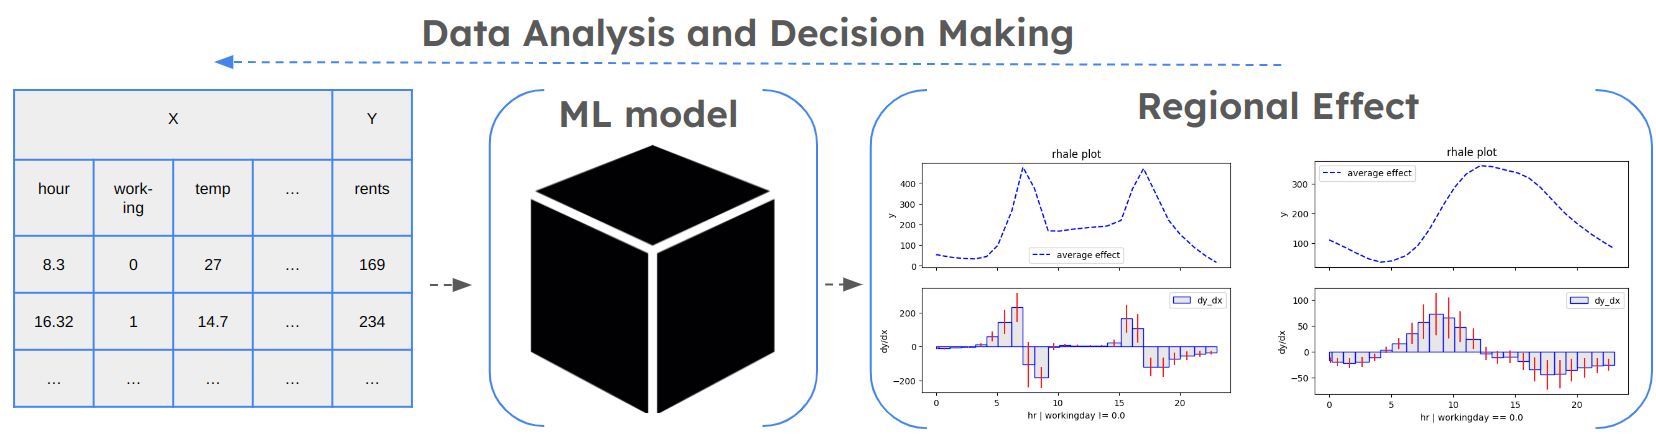
\includegraphics[width=\textwidth]{figures/concept_image.png}
    \caption{Data analysis and decision making pipeline: Utilizing regional effect plots to extract insights from tabular data.}
    \label{fig:concept_figure}
\end{figure*}

\section{Regional RHALE}

r-RHALE builds on two papers. Gkolemis et al. (2023)~\citep{gkolemis2023rhale} introduced RHALE, a global effect method for differentiable black-box models that improves on ALE by being faster and computing heterogeneity. As we will show below, the heterogeneity is crucial quantity for subregion detection. Herbinger et al. (2023)~\citep{herbinger2023decomposing} proposed a generic framework for transforming global effect methods to regional, and applied it to PDP\cite{friedman_predictive_2008}, ALE\cite{apley_visualizing_2020}, and SHAP-DP\cite{lundberg2017unified}. This paper integrates these approaches.

\begin{figure*}
  \centering
  \begin{subfigure}[t]{0.32\textwidth}
  \centering
  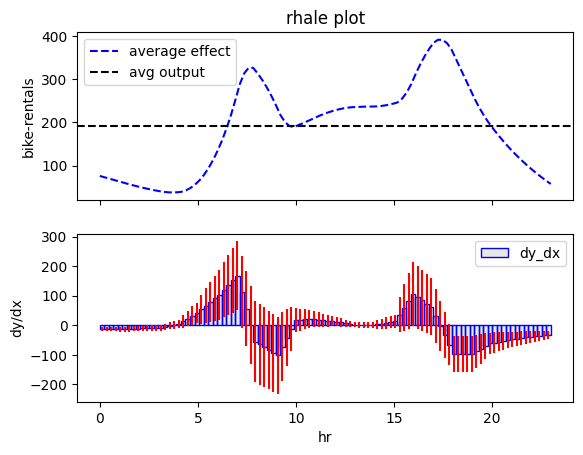
\includegraphics[width=\linewidth]{figures/running_example/01_bike_sharing_dataset_23_1.png}
  \caption{Global effect}
  \label{subfig:global}
  \end{subfigure}
  \begin{subfigure}[t]{0.32\textwidth}
  \centering
  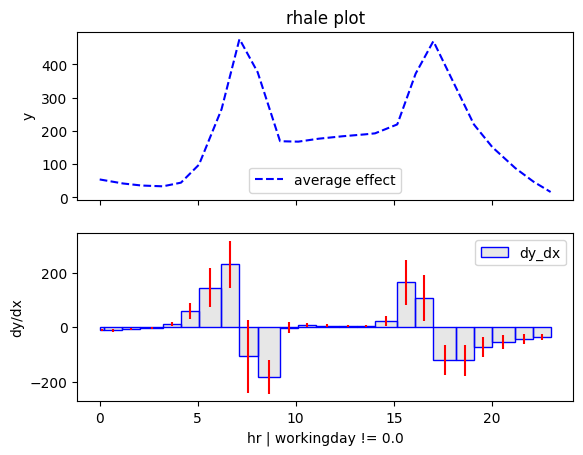
\includegraphics[width=\linewidth]{figures/running_example/01_bike_sharing_dataset_29_1.png}
  \caption{Effect on working days}
  \label{subfig:regional_a}
  \end{subfigure}
  \begin{subfigure}[t]{0.32\textwidth}
  \centering  
  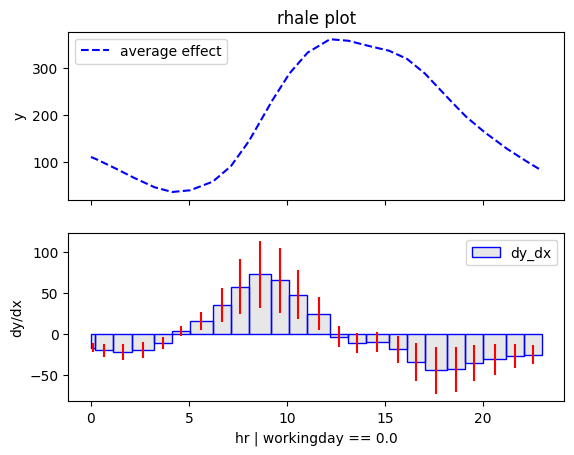
\includegraphics[width=\linewidth]{figures/running_example/01_bike_sharing_dataset_29_0.png}
  \caption{Effect on non-working days}
  \label{subfig:regional_b}
  \end{subfigure}
  \caption{r-RHALE applied to the bike-sharing dataset; (a) global effect of feature hour on the bike-rentals (b) regional effect on working days (c) regional effect on non-working days.}
  \label{fig:main-concept}
\end{figure*}

\paragraph{Notation.}

Let \(\mathcal{X} \in \mathbb{R}^d\) be the \(d\)-dimensional feature space, \(\mathcal{Y}\) the target space and
\(f(\cdot) : \mathcal{X} \rightarrow \mathcal{Y}\) the black-box function.
We use index \(\mathtt{s} \in \{1, \ldots, d\}\) for the feature of interest and \(\mathtt{C} = \{1, \ldots, d\} - s\) for the indices of all the other features.
For convenience, we use \((x_s, \xc)\) to denote the input vector \((x_1, \cdots , x_s, \cdots, x_D)\),
\((X_s, \Xc)\) instead of \((X_1, \cdots , X_s, \cdots, X_D)\) for random variables and
$\mathcal{X}_s, \mathcal{X}_{c}$ for the feature space and its complement, respectively.
The training set \(\mathcal{D} = \{(\xb^i, y^i)\}_{i=1}^N\) is sampled
i.i.d.\ from the distribution \(\mathbb{P}_{X,Y}\).

\paragraph{globalRHALE.}

RHALE esitmates the effect of feature $x_s$ on the output $y$ (Figure~\ref{subfig:global}), as:

\begin{equation}
  \label{eq:rhale-approximation}
f(x_s) = \underbrace{\sum_{k=1}^{k_{x_s}} \underbrace{\frac{z_k - z_{k-1}}{ \left | \mathcal{S}_k \right |} \sum_{i: \xb^i \in \mathcal{S}_k} \overbrace{\frac{\partial f}{\partial x_s} (x_s^i, \xci)}^{\text{instance effect}}}_{\mu_k (\text{interval effect})}}_{\text{global effect}}
\end{equation}

\noindent
The feature axis $x_s$ is divided into $K_s$ variable-size intervals $\{\mathcal{Z}_k\}_{k=1}^{K_s}$, where each interval spans $[z_{k-1}, z_k)$. Let $\mathcal{S}_k$ be the set of instances with the $s$-th feature in the $k$-th interval, i.e., $\mathcal{S}_k = \{ x^{(i)} : z_{k-1} \leq x^{(i)}_s < z_k \}$. The interval boundaries are determined by solving an optimization problem as described in Gkolemis et al. (2023).

To understand Eq.~(\ref{eq:rhale-approximation}), we proceed step by step. The instance effect, $\frac{\partial f}{\partial x_s} (x_s^i, \xci)$, measures the change in the output when the $s$-th feature changes slightly from $(x_s^i, \xci)$ to $(x_s^i + \delta, \xci)$. We then average the instance effects for all instances in the $k$-th bin to obtain the bin effect, $\mu_k$. The global effect is the sum of the bin effects.

\paragraph{Heterogeneity.}

Heterogeneity measures the deviation of instance effects from the bin effect:

\begin{equation}
  \label{eq:rhale-approximation-heterogeneity}
  H_s = \sum_{k=1}^{K_s} \frac{z_k - z_{k-1}}{|\mathcal{S}_k|}\sum_{i: \xb^i \in \mathcal{S}_k} \left [ \frac{\partial f}{\partial x_s} (x_s^i, \xci) - \mu_k \right ]^2
\end{equation}

\noindent
Zero heterogeneity indicates that the effect of $x_s$ on the output is independent of other features, i.e., \( f(\xb) = f_s(x_s) + f_c(\xc) \). In this ideal case, the feature effect explanation is reliable for all instances. As heterogeneity increases, the feature effect explanation becomes less accurate for individual instances, reflecting a stronger dependence on other features $\xc$. 

For example, the effect of hour on bike rentals significantly depends on the day type, resulting in high heterogeneity and inaccurate average explanations for non-working days. By splitting data into working and non-working days, regional effects reduce heterogeneity, providing reliable explanations within each subregion.

\paragraph{r-RHALE.}

Regional effects aim to identify subregions with reduced heterogeneity by conditioning on one ore more of the features in \( \mathtt{C} \). For continuous features, this condition is based on whether the feature value is above or below a threshold \( \tau \), and for categorical features, whether it equals or differs from \( \tau \). A CART-based algorithm iterates over all features in \( \xb_c \) and tests various thresholds \( \tau \) to find the one that maximally reduces heterogeneity.
r-RHALE combines the heterogeneity measure from Eq.~(\ref{eq:rhale-approximation-heterogeneity}) with this CART-based algorithm, as detailed in~\cite{herbinger2023decomposing, gkolemis2024effector}.

\paragraph{Computational Advantage.}

r-RHALE offers a computational advantage over other methods due to its approach to computing heterogeneity. According to Eq.~(\ref{eq:rhale-approximation-heterogeneity}), the term \( \frac{\partial f}{\partial x_s} (x_s^i, \xci) \) needs to be computed only once for all instances. When executed in a batched manner with support for automatic differentiation, the computational time is comparable to a single evaluation of \( f \). In contrast, other methods require multiple evaluations of \( f \) to compute regional effects, resulting in slower execution times, especially for complex and computationally intensive functions \( f \).

\section{Synthetic Examples}

We test our approach on two synthetic examples. The synthetic example of Section~\ref{sec:efficiency} demonstrates that r-RHALE is faster than the existing methods and the example of Section~\ref{sec:correlated-features}, unlike r-PDP, it handles well tabular datasets with correlated features.

\subsection{Execution time comparison}
\label{sec:efficiency}


In this example, we show that r-RHALE executes significantly faster than r-PDP and r-ALE.
We do not include r-SHAPDP in the comparison, because its execution time is prohibitive high, e.g., more than 30 minutes, even for relatively light models and datasets. In the example, we observe that r-RHALE executes fast even under a (a) slow-inference black-box model and (b) a large tabular dataset.

\paragraph{Slow-inference black-box model:}

We generate a dataset with $N=10^4$ instances, $D=10$ features and train deep neural networks (DNN) with layers ranging from $L=3$ to $L=20$. More layers means bigger inference time, so our findings generalize to any slow-inference black-box model.

In Figure~\ref{fig:efficiency_heavy_model}, we observe that r-RHALE's execution time increases at a slower rate compared to r-ALE and r-PDP. Even for complex models like DNNs with 20 layers, r-RHALE requires less than 15 seconds to generate regional effect plots for a single feature. This translates to approximately 4-5 minutes for a typical tabular dataset with 20 features. In contrast, r-PDP requires about 4 minutes per feature, totaling roughly an hour for all features, while r-ALE needs about 1 minute per feature, resulting in approximately 20 minutes for all features.

\begin{figure}
    \centering
    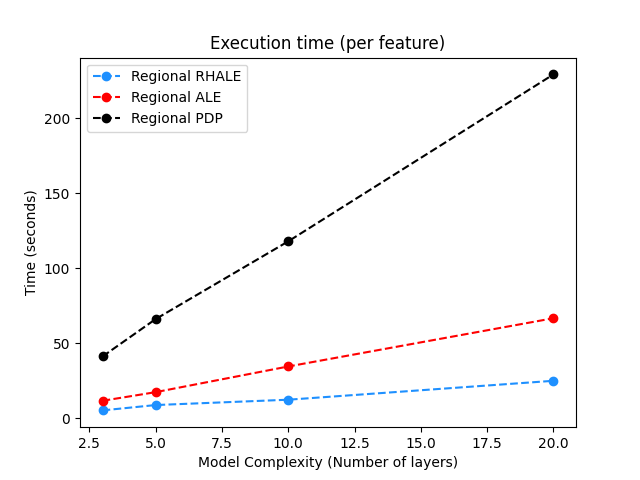
\includegraphics[width=.49\textwidth]{figures/simulation_2/efficiency_layers.png}
    \caption{Execution time applied to neural networks of varying number of layers, i.e., varying inference times.}
    \label{fig:efficiency_heavy_model}
\end{figure}

\paragraph{Large tabular dataset:}

We define a deep neural network (DNN) with \( L = 5 \) layers and a synthetic dataset with \( D = 20 \) features and a varying number of instances \( N \in \{10^3, 10^4, 10^5\} \) (log scale).

In Figure~\ref{fig:efficiency_nof_instances}, we observe that r-RHALE's execution time increases at a slower rate compared to r-ALE and r-PDP. r-RHALE is more than twice as fast as r-ALE and ten times faster than r-PDP. For large datasets, this translates to a speed-up of 20 minutes compared to r-ALE and 2 hours compared to r-PDP. The efficiency gain would be even more pronounced with a heavier black-box model, as demonstrated in the previous example.

\begin{figure}
    \centering
    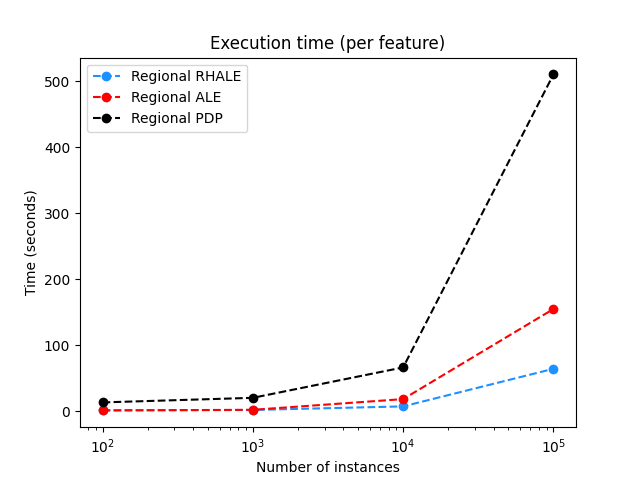
\includegraphics[width=.49\textwidth]{figures/simulation_2/efficiency_samples.png}
    \caption{Execution time of regional effect methods applied on datasets with a varying number of instances (log scale).}
    \label{fig:efficiency_nof_instances}
\end{figure}


\subsection{Correlated Features}
\label{sec:correlated-features}

In this example, we demonstrate that, unlike r-PDP, r-RHALE handles well tabular datasets with correlated features.

We use the model \( y = 3x_1I_{x_3 > 0} - 3x_1I_{x_3 \leq 0} + x_3 \) with two different data-generating distributions. In the non-correlated setting, all variables are uniformly distributed, \( x_i \sim \mathcal{U}(-1,1) \). In the correlated setting, \( x_1 \) and \( x_2 \) maintain the same distributions, but \( x_3 = x_1 \).

These two versions illustrate that r-PDP produces the same regional effect regardless of correlations, while r-RHALE accurately distinguishes between the two cases. We focus on the effect (both global and regional) of \( x_1 \) on \( y \).

\paragraph{Non-correlated setting.}

The effect of \( x_1 \) arises from the interaction terms \( 3x_1I_{x_3>0} \) and \( 3x_1I_{x_3\leq0} \). The global effect will be \( 3x_1 \) when \( x_3 > 0 \) (half the time, given \( x_3 \sim \mathcal{U}(-1,1) \)) and \( -3x_1 \) when \( x_3 \leq 0 \) (the other half). This results in an overall zero global effect with high heterogeneity. By splitting into two subregions, \( x_3 > 0 \) and \( x_3 \leq 0 \), we obtain two regional effects, \( 3x_1 \) and \( -3x_1 \), each with zero heterogeneity.

In Figure~\ref{fig:synthetic-1-uncorrelated}, both r-PDP and r-RHALE correctly identify the global effect. The global effect is zero but with high heterogeneity, indicated by the two red lines in the r-PDP plot (Figure~\ref{subfig:global_pdp}) and the red bars in the r-RHALE plot (Figure~\ref{subfig:global_rhale}). Due to space limitations, we do not illustrate the regional effects, which, in both cases, match the ground truth.

\begin{figure}[t]
    \centering
    \begin{subfigure}[b]{0.24\textwidth}
        \centering
        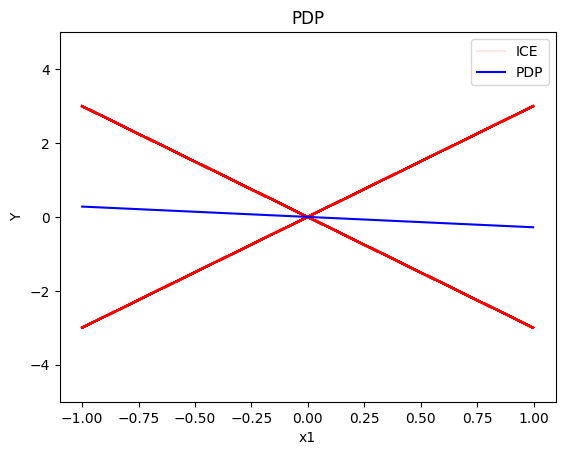
\includegraphics[width=\textwidth]{figures/simulation_1/uncor_global_pdp.png}
        \caption{Global PDP ($x_1$)}
        \label{subfig:global_pdp}
    \end{subfigure}
    \begin{subfigure}[b]{0.24\textwidth}
        \centering
        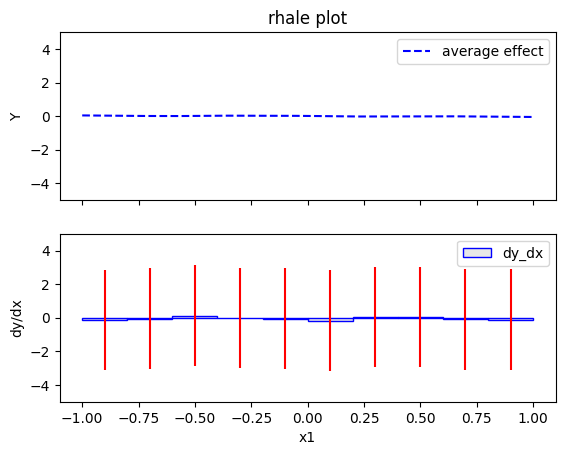
\includegraphics[width=\textwidth]{figures/simulation_1/uncor_global_rhale.png}
        \caption{Global RHALE ($x_1$)}
        \label{subfig:global_rhale}
    \end{subfigure}
    \caption{Global plots for the non-correlated setting.}
    \label{fig:synthetic-1-uncorrelated}
  \end{figure}

\paragraph{Correlated setting.}

In the correlated case, with \( x_3 = x_1 \), the effect becomes \( y = 3x_1I_{x_1 > 0} - 3x_1I_{x_1 \leq 0} \). This is because the interaction terms simplify to \( 3x_1I_{x_1 > 0} \) and \( -3x_1I_{x_1 \leq 0} \). When \( x_1 > 0 \), \( x_3 > 0 \), so only the \( 3x_1 \) term is active. Similarly, when \( x_1 \leq 0 \), \( x_3 \leq 0 \), making only the \( -3x_1 \) term active.

In Figure~\ref{fig:synthetic-1-correlated}, we observe that only r-RHALE correctly estimates the global and regional effects. r-RHALE (Figure~\ref{subfig:global_rhale_correlated}) accurately computes the effect as \( 3x_1I_{x_1 > 0} - 3x_1I_{x_1 \leq 0} \) with no heterogeneity and does not identify subregions. In contrast, r-PDP (Figure~\ref{subfig:global_pdp_correlated}) treats the features as independent, resulting in the same global effect as in the uncorrelated case and incorrectly identifying subregions for \( x_3 > 0 \) and \( x_3 \leq 0 \).


\begin{figure}[t]
    \centering
    \begin{subfigure}[b]{0.24\textwidth}
        \centering
        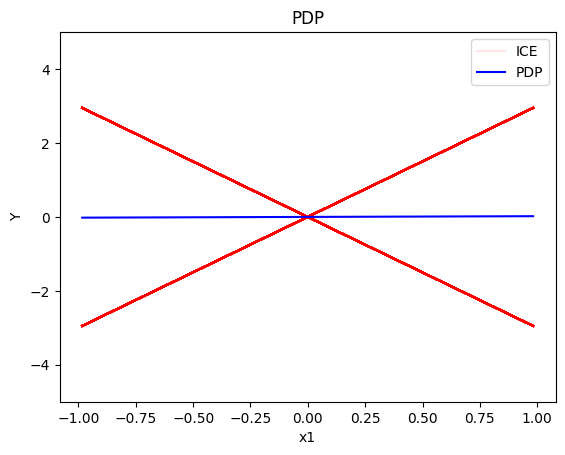
\includegraphics[width=\textwidth]{figures/simulation_1/cor_global_pdp.png}
        \caption{Global PDP ($x_1$)}
        \label{subfig:global_pdp_correlated}
    \end{subfigure}
    \begin{subfigure}[b]{0.24\textwidth}
        \centering
        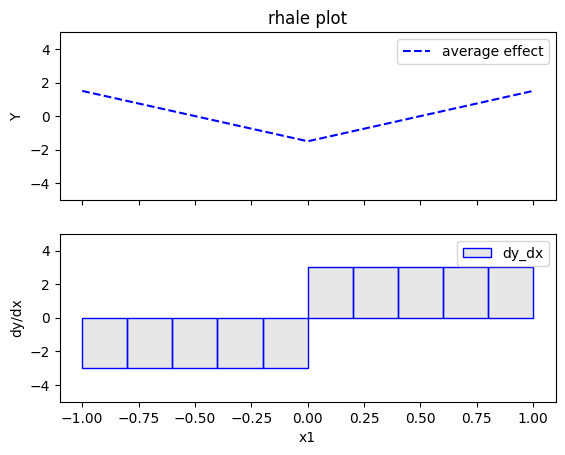
\includegraphics[width=\textwidth]{figures/simulation_1/cor_global_rhale.png}
        \caption{Global RHALE ($x_2$)}
        \label{subfig:global_rhale_correlated}
    \end{subfigure}
    \caption{Global plots for the correlated setting.}
    \label{fig:synthetic-1-correlated}
  \end{figure}
  
  
\section{Conclusion and Future Work}

In this paper, we introduce a novel method for extracting insights from tabular data. Our approach involves first fitting a black-box model and then explaining its predictions using a regional effect method. The insights gained from the regional effect can then be applied to support decision-making processes.

To this end, we propose r-RHALE, an innovative regional effect method that builds upon the strengths of the global effect RHALE. r-RHALE offers significantly improved efficiency compared to existing methods and effectively handles datasets with correlated features.

\bibliography{regional_rhale.bib}

\end{document}

%%
%% End of file
